\documentclass[12pt,a4paper]{article}

\usepackage[utf8]{inputenc}
\usepackage[ngerman]{babel}
\usepackage[T1]{fontenc}
\usepackage{amsmath}
\usepackage{amsfonts}
\usepackage{amssymb}
\usepackage{graphicx}
\usepackage[left=2cm,right=2cm,top=2cm,bottom=2cm]{geometry}
\usepackage{multicol}
\usepackage{booktabs}
\usepackage[hidelinks]{hyperref}
\usepackage{tikz}
\usepackage{pgfplots}
\usepackage{blindtext}
\usepackage{array}
\usepackage{multirow}
\usepackage{bigdelim}
\usepackage{colortbl}
\usepackage{fancyhdr} 
\usepackage{tabularx}
\usepackage{xcolor}
\usepackage{color}
\usetikzlibrary{decorations.text}
\usetikzlibrary{tikzmark}
\pagestyle{fancy} 
	\fancyhf{} 
	\fancyhead[L]{
\includegraphics[scale=0.05]{Bilder/dhbw.png}} 
	\fancyhead[C]{\slshape Netztechnik} 
	\fancyhead[R]{\slshape LaTeX Version}
	\fancyfoot[C]{\thepage}
\usepackage{helvet}
\renewcommand{\familydefault}{\sfdefault}

\title{Netztechnik}
\author{\slshape Robin Rausch, Florian Maslowski}
\date{\slshape \today}

\begin{document}
	\pagenumbering{Roman}
	\maketitle
	\tableofcontents
	\newpage
	\pagenumbering{arabic}
	\section{Grundlagen}
		\subsection{OSI-7-Schichten-Modell}
			\textbf{Merkhilfe:} Please Do Not Throw Salami Pizza Away.\\
			%image of OSI-Modell
		\subsection{Protokolle (+Zuordnung)}

	\section{Netze}
		\subsection{Netzwerk-Topologien}

		\subsection{Netzwerk-Technologien}
			\begin{description}
				\item[Repeater] Verstärkt Eingangssignal auf Ausgang, OSI-Schicht 1
				\item[Hub] Multiport Repeater, OSI-Schicht 1
				\item[Bridge] Verbindet 2 Netze, arbeitet mit MAC-Adressen, OSI-Schicht 2 
				\item[Switch] Schlauer Hub. Verstärkt nur an richtigen Port. Arbeitet mit MAC-Adressen, OSI-Schicht 2 
				\item[Router] Verbindet Netze, arbeitet mit IP-Adressen, OSI-Schicht 3
				\item[Gateway] Verbindet Netze, arbeitet auf allen OSI-Schichten, Protokollunabhängig 
			\end{description}

		\subsection{Subnetting}

		\subsection{Switch}
			\subsubsection{Spanning Tree}
				Switche haben Hierarchie beim Weiterleiten von Paketen. Kleine Priorität ist besser. Falls Priorität gleich, entscheidet höhere MAC-Adresse die bevorzugte Switch\\
				Switche geben Pakete nur an Switche mit geringerer Priorität oder höherer MAC-Adresse weiter. Beste Switch in der Vernetzung wird zum Root.\\
				Es gibt dabei 3 Arten von Ports an den Switches:
				\begin{description}
					\item[Root-Port] Zur Root-Switch
					\item[Designated-Port] Zu Switch mit besserer Priorität oder höherer MAC-Adresse als die eigene
					\item[Blocking-Port] Zu Switches, welche weniger bevorzugt sind als sie selbst 
				\end{description}
				In Untenstehender Skizze ist Switch B die Root-Switch und alle Ports, die zu ihr führen, sind Root-Ports.\\
				Da die restlichen Switche die gleiche Priorität haben, wird die höchste MAC-Adresse bevorzugt. \\
				Dadurch sind die Ports zu Switch A die Blocking-Ports und die von D zu A und C ebenfalls. \\
				Ports an Root-Switch sind alle designated.\\
				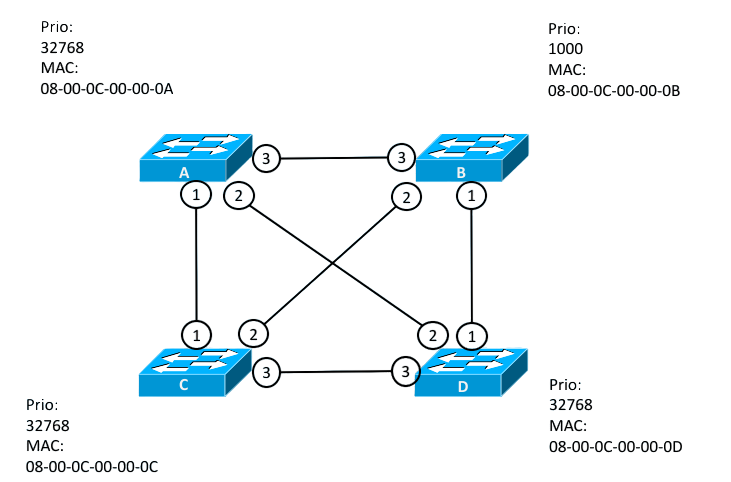
\includegraphics[scale=0.5]{Bilder/RouterVermascht.png}

	\section{Kabel}

		\subsection{Kabelarten:}
		\begin{description}
			\item[Twisted-Pair] Verdrillte Paare, um geringes Nebensprechen mit hoher Übertragbarkeit zu erreichen.
			\item[LWL] Lichtwellenleiter/Glasfaserkabel hohe Geschwindigkeit, teuer, Aufwand in Spannung zurückzuwandeln.
		\end{description}

		\subsection{Verkablungsarten:}
		\begin{description}
			\item[Primarverkabelung: ] Für Verkabelung von Gebäuden mit LWL
			\item[Sekundärverkabelung: ] Für Verkabelung von Etagen mit LWL
			\item[Tertiärverkabelung: ] Für Verkabelung innerhalb einer Etage mit Kupferkabel
		\end{description}

	\section{Codierung}
		\subsection{Huffmann-Codierung}
			Algorythmus zum \textbf{Komprimieren} von Dateien.\\
			\textbf{Idee:} Häufige Zeichen kurze Bit-Codierung, sodass Binär-Codierung möglichst kurz ist.
			\begin{enumerate}
				\item \textbf{Tabelle} mit vorkommenden Zeichen und deren Häuffigkeit erstellen
				\item \textbf{Binärbaum} mit Zeichen erstellen. Zeichen nach Häufigkeit sortiert. Zeichen mit geringster Häufigkeit zusammenfassen. Zusammengefasste zeichen weiter vereinen bis Baum vollständig ist\\
				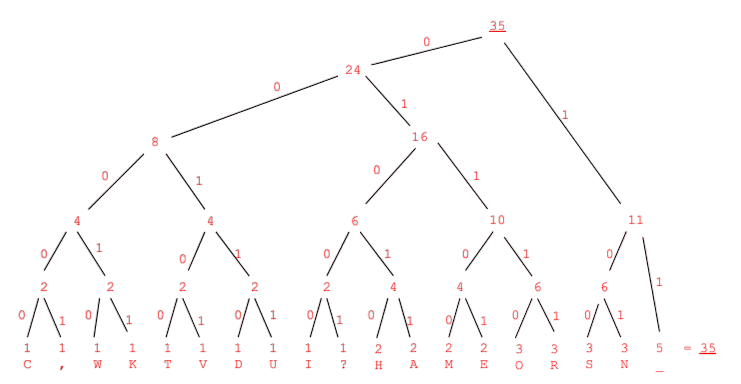
\includegraphics[scale=0.4]{Bilder/Huffmann-Baum.png}
				\item \textbf{Codierung} der Zeichen aus Binärbaum lesen und in Tabelle schreiben
			\end{enumerate}
\end{document}
